\section{电子在周期势场中的运动}

\begin{quotation}
``传统半导体与光子晶体相结合的集成电路将意味着光电子学上小型化的极限。''
\end{quotation}


\begin{figure}[h]
\begin{center}
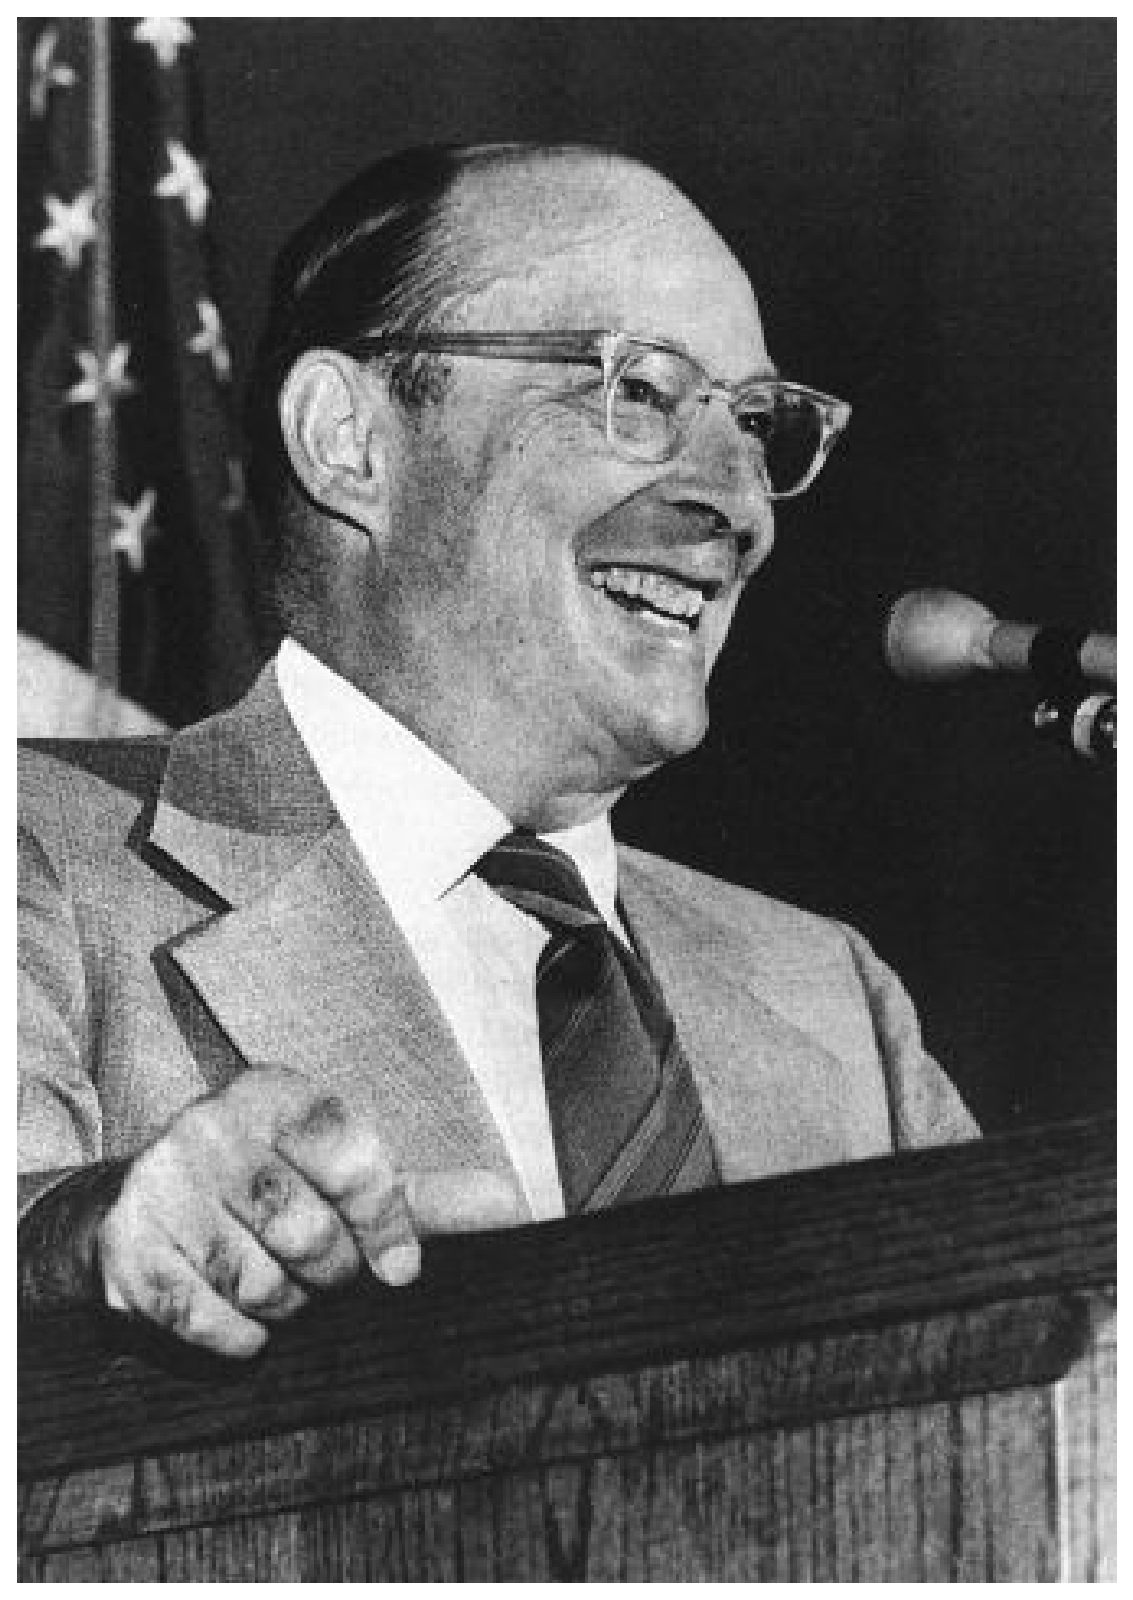
\includegraphics[clip,width=6cm]{Symmetry/bardeen.ps}
\caption{巴丁}
\end{center}
\end{figure}


\subsection{电子在周期势场中的运动}

\index{Periodic potential: 周期势场}

我们讨论一维情形,设$V(x)$是周期势,满足:$V(x + a) = V(x)$;

(1)证明$\exp \left[ {a{\textstyle{d \over {dx}}}} \right]\psi (x) = \psi (x + a)$

左边:$\exp \left[ {a{\textstyle{d \over {dx}}}} \right]\psi (x) = \sum\limits_{n = 0}^\infty  {\frac{{a^n {\textstyle{{d^n } \over {dx^n }}}}}{{n!}}} \psi (x) = \sum\limits_{n = 0}^\infty  {\frac{{a^n \psi ^{(n)} (x)}}{{n!}}} $

右边:$\psi (x + a) = \sum\limits_{n = 0}^\infty  {\frac{{a^n \psi ^{(n)} (x)}}{{n!}}} $

可以定义平移算符为:$\widehat T(a) = \exp \left[ {a\frac{d}{{dx}}} \right] = \exp \left[ {a\frac{i}{\hbar }\frac{\hbar }{i}\frac{d}{{dx}}} \right] = \exp \left[ {\frac{{i\widehat p \cdot a}}{\hbar }} \right]$


一般而言平移算符可写为:$\widehat T\left( {\mathord{\buildrel{\lower3pt\hbox{$\scriptscriptstyle\rightharpoonup$}}
\over r} } \right) = \exp \left( {\frac{{i\widehat{\mathord{\buildrel{\lower3pt\hbox{$\scriptscriptstyle\rightharpoonup$}}
\over p} } \cdot \mathord{\buildrel{\lower3pt\hbox{$\scriptscriptstyle\rightharpoonup$}}
\over r} }}{\hbar }} \right)$,这里$\vec r$表示平移的参数,而不是位置算符,所以$\widehat{\vec p} \cdot \vec r = \vec r \cdot \widehat{\vec p}$

(2)证明哈密顿算符:$\hat H =  - \frac{{\hbar ^2 }}{{2m}}\frac{{d^2 }}{{dx^2 }} + V\left( x \right)$与平移算符$\widehat T(a)$对易;

$\left[ {\widehat T\left( a \right),\widehat H} \right] = \left[ {\widehat T\left( a \right), - \frac{{\hbar ^2 }}{{2m}}\frac{{d^2 }}{{dx^2 }} + V\left( x \right)} \right]$

$\widehat T\left( a \right) = \sum\limits_n {\frac{1}{{n!}}\left( {\frac{{ia}}{\hbar }} \right)} ^n \widehat p^n $,所以:$\left[ {\widehat T(a),\frac{{\widehat p^2 }}{{2m}}} \right] = 0$

$\begin{array}{l}
 \left[ {\widehat T(a),V(x)} \right]\psi (x) = \widehat T(a)V(x)\psi (x) - V(x)\widehat T(a)\psi (x) \\
  = V\left( {x + a} \right)\psi \left( {x + a} \right) - V\left( x \right)\psi \left( {x + a} \right) \\
 \end{array}$

利用:$V(x + a) = V(x)$;

$\left[ {\widehat T\left( a \right),V\left( x \right)} \right] = 0$

所以:$\left[ {\widehat T\left( a \right),\widehat H} \right] = \left[ {\widehat T\left( a \right),\frac{{\widehat p^2 }}{{2m}} + V\left( x \right)} \right] = 0$


(3)证明:一维运动电子,设$\psi _1 \left( x \right),\psi _2 \left( x \right)$都是薛定谔方程:

\begin{center}
$\left[ { - \frac{{\hbar ^2 }}{{2m}}\frac{{d^2 }}{{dx^2 }} + V\left( x \right)} \right]\psi \left( x \right) = E\psi \left( x \right)$
\end{center}

的解;且都是相同能量本征值$E$的解,证明:$\psi _1 \psi _2 ^\prime   - \psi _2 \psi _1 ^\prime   = {\rm{Const}}$

对$\psi _1, \psi _2$分别列出薛定谔方程:

$\begin{array}{l}
 \psi _1 ^{\prime \prime }  + \frac{{2m}}{{\hbar ^2 }}\left[ {E - V\left( x \right)} \right]\psi _1  = 0 \\
 \psi _2 ^{\prime \prime }  + \frac{{2m}}{{\hbar ^2 }}\left[ {E - V\left( x \right)} \right]\psi _2  = 0 \\
 \end{array}$


$\begin{array}{l}
 \psi _1 ^{\prime \prime } \psi _2  + \frac{{2m}}{{\hbar ^2 }}\left[ {E - V\left( x \right)} \right]\psi _1 \psi _2  = 0 \\
 \psi _2 ^{\prime \prime } \psi _1  + \frac{{2m}}{{\hbar ^2 }}\left[ {E - V\left( x \right)} \right]\psi _2 \psi _1  = 0 \\
 \end{array}$

两式相减:$\psi _1 \psi _2 ^{\prime \prime }  - \psi _2 \psi _1 ^{\prime \prime }  = 0$

即:$\left( {\psi _1 \psi _2 ^\prime   - \psi _2 \psi _1 ^\prime  } \right)^\prime   = 0$

所以:$\psi _1 \psi _2 ^\prime   - \psi _2 \psi _1 ^\prime   = {\rm{Const}}$

(4)Floque定理: $\psi \left( {x + a} \right) = \widehat T\left( a
\right)\psi \left( x \right) = e^{i{\textstyle{{\widehat p \cdot a}
\over \hbar }}} \psi \left( x \right) = e^{iKa} \psi \left( x
\right)$

(4.1)一维定态薛定谔方程是二阶常微分方程,对每个本征值$E$,一般存在两个线性无关的解(如:无限势阱中属于$E_n$的$\sin nx,\cos nx$), $u_1 (x),u_2 (x)$, 由于$\left[ {\widehat T(a),\widehat H} \right] = 0$, 存在线性无关解$u_1 (x),u_2 (x)$同时也是$\widehat T\left( a \right)$的本征函数:$\widehat T(a)u_i (x) = u_i (x + a) = \lambda _i u_i (x)$; $i = 1,2$

同样:$\widehat T(a)u_i^* (x) = u_i^* (x + a) = \left( {\lambda _i u_i (x)} \right)^*  = \lambda _i^* u_i^* (x)$

即$\lambda _i ^* $也是平移算符$\widehat T(a)$的本征函数,而且$\lambda _i ^* $必须与$\lambda _i$相同;

所以:$\lambda _1 ^*  = \lambda _1 ,\lambda _2 ^*  = \lambda _2 $,或者:$\lambda _1 ^*  = \lambda _2 ,\lambda _2 ^*  = \lambda _1 $

(4.2)利用:$\psi _1 \psi _2 ^\prime   - \psi _2 \psi _1 ^\prime   = {\rm{Const}}$

$\frac{d}{{dx}}\left[ {u_1 u_2 ^\prime   - u_2 u_1 ^\prime  } \right] = \frac{d}{{dx}}W\left( x \right) = 0$, $W\left( x \right) = {\rm{Const}}$

所以:$W\left( x \right) = W\left( {x + a} \right) = \lambda _1 \lambda _2  = 1$

综合(4.1) (4.2)结果:

$\lambda _1 ^*  = \lambda _1 ,\lambda _2 ^*  = \lambda _2 $, $\lambda _i  \in {\rm{Real}}$, $\psi \left( {x + na} \right) = \lambda _i ^n \psi \left( x \right),\psi \left( {x - na} \right) = \frac{1}{{\lambda _i ^n }}\psi \left( x \right)$

所以:$\left| {\lambda _i } \right| > 1$或$\left| {\lambda _i } \right| < 1$会导致波函数在$x \to \infty $
或$x \to  - \infty $发散,这是不允许的;

$\lambda _1 ^*  = \lambda _2 ,\lambda _2 ^*  = \lambda _1 $,$\lambda _1 \lambda _2  = \lambda _1 \lambda _1 ^*  = \lambda _2 ^* \lambda _2  = 1$,所以$\left| {\lambda _i } \right|^2  = 1$

可以表示为指数的形式:$\lambda _1  = e^{iKa} ,\lambda _2  = e^{ - iKa} ,K \in {\rm{Real}}$

即:$u_1 \left( {x + a} \right) = e^{iKa} u_1 \left( x \right),u_2 \left( {x + a} \right) = e^{ - iKa} u_2 \left( x \right)$

(5)Bloch定理:如令$\psi \left( x \right) = e^{iKx} \phi _K \left( x \right)$,可证明$\phi _K \left( x \right)$是周期函数,周期与势场周期相同,$\phi _K \left( {x + a} \right) = \phi _K \left( x \right)$,$K \in {\rm{Real}}$,称为Bloch波数;

\index{Bloch's theorem: 布洛赫定理}

由Floque定理,波函数可表示为:$\psi \left( {x + a} \right) = e^{iKa} \psi \left( x \right)$

把$\psi \left( x \right) = e^{iKx} \phi _K \left( x \right)$代入方程两边:

$e^{iK\left( {x + a} \right)} \phi _K \left( {x + a} \right) = e^{iKa} e^{iKx} \phi _K \left( {x + a} \right) = e^{iKa} e^{iKx} \phi _K \left( x \right)$

所以:$\phi _K \left( {x + a} \right) = \phi _K \left( x \right)$

(6)能带结构:

\index{Band structure: 能带结构}

周期势场中,当$x \in \left[ {0,a} \right]$,波函数可表示为两个线性无关解的迭加:


$\psi \left( x \right) = Au_1 \left( x \right) + Bu_2 \left( x \right)$

由Floque定理,区间平移$a$:$\psi \left( {x + a} \right) = e^{iKa} \psi \left( x \right)$

即:$\psi \left( x \right) = e^{iKa} \psi \left( {x - a} \right) = e^{iKa} \left[ {Au_1 \left( {x - a} \right) + Bu_2 \left( {x - a} \right)} \right]$

$x = a$时,连续性条件:$\psi ,\psi '$连续

$\left\{ \begin{array}{l}
 Au_1 \left( a \right) + Bu_2 \left( a \right) = e^{iKa} \left[ {Au_1 \left( 0 \right) + Bu_2 \left( 0 \right)} \right] \\
 Au_1 ^\prime  \left( a \right) + Bu_2 ^\prime  \left( a \right) = e^{iKa} \left[ {Au_1 ^\prime  \left( 0 \right) + Bu_2 ^\prime  \left( 0 \right)} \right] \\
 \end{array} \right.$

$A, B$有解的条件:

$\left| {\begin{array}{*{20}c}
   {u_1 (a) - e^{iKa} u_1 (0)} & {u_2 (a) - e^{iKa} u_2 (0)}  \\
   {u_1 ^\prime  (a) - e^{iKa} u_1 ^\prime  (0)} & {u_2 ^\prime  (a) - e^{iKa} u_2 ^\prime  (0)}  \\
\end{array}} \right| = 0$

展开为:

\begin{eqnarray*}
0 & = & \left( {u_1 (a) - e^{iKa} u_1 (0)} \right)\left( {u_2 ^\prime  (a) - e^{iKa} u_2 ^\prime  (0)} \right) - \\
{} & {} & \left( {u_2 (a) - e^{iKa} u_2 (0)} \right)\left( {u_1 ^\prime  (a) - e^{iKa} u_1 ^\prime  (0)} \right) \\
{} & = & u_1 (a)u_2 ^\prime  (a) + e^{i2Ka} u_1 (0)u_2 ^\prime  (0) - e^{iKa} u_1 (0)u_2 ^\prime  (a) - e^{iKa} u_1 (a)u_2 ^\prime  (0) -  \\
{} & {} &  \left[ {u_2 (a)u_1 ^\prime  (a) + e^{i2Ka} u_2 (0)u_1 ^\prime  (0) - e^{iKa} u_2 (0)u_1 ^\prime  (a) - e^{iKa} u_2 (a)u_1 ^\prime  (0)} \right] \\
{} & = & W(a) + e^{i2Ka} W(0) - e^{iKa} \left[ {u_1 (0)u_2 ^\prime  (a) + u_1 (a)u_2 ^\prime  (0)} \right] + \\
{} & {} & e^{iKa} \left[ {u_2 (0)u_1 ^\prime  (a) + u_2 (a)u_1 ^\prime  (0)} \right]
\end{eqnarray*}



$W(a) = W(0) = u_1 u_2 ^\prime   - u_2 u_1 ^\prime   = {\rm{Const}}$

定义:

$\begin{array}{l}
 U_1  = u_1 (0)u_2 ^\prime  (a) + u_1 (a)u_2 ^\prime  (0) \\
 U_2  = u_2 (0)u_1 ^\prime  (a) + u_2 (a)u_1 ^\prime  (0) \\
 \end{array}$

行列式简化为:$0 = W\left( {1 + e^{i2Ka} } \right) - e^{iKa} U_1  + e^{iKa} U_2 $

$W\left( {1 + e^{i2Ka} } \right) = e^{iKa} \left( {U_1  - U_2 } \right)$

即:$W\left( {e^{ - iKa}  + e^{iKa} } \right) = U_1  - U_2 $

$ \Rightarrow 2W\cos Ka = U_1  - U_2  \Rightarrow \cos Ka = \frac{{U_1  - U_2 }}{{2W}}$

由于:$\left| {\cos Ka} \right| \le 1$,即:$\left| {\frac{{U_1  - U_2 }}{{2W}}} \right| \le 1$,这个表达式是对粒子能量本征值的限制,即只有部分能量是允许的,这样就形成了能带结构;允许的称为导带,禁止的称为禁带,交界处就在$\cos Ka =  \pm 1$的点,即:$Ka = n\pi $\footnote{参考曾谨言《量子力学 卷I》第150页}。


\subsection{Kronig-Penny模型}

(7)设周期势场:$V(x) =  - V_0 \sum\limits_{n =  - \infty }^{ + \infty } {\delta \left( {x + na} \right)} $,$V_0  > 0$,求本征值条件;(固体物理中能带的Kronig-Penny模型)

考虑:$x \in \left( {0,a} \right)$,$V(x) = 0$,薛定谔方程:$ - \frac{{\hbar ^2 }}{{2m}}\frac{{d^2 }}{{dx^2 }}\psi  = E\psi $,$\psi '' + \frac{{2mE}}{{\hbar ^2 }}\psi  = 0$

$\psi _1 \left( x \right) = Ae^{ikx}  + Be^{ - ikx} $,$k^2  = \frac{{2mE}}{{\hbar ^2 }}$

考虑:$x \in \left( {a,2a} \right)$,由Floque定理,波函数可表示为:$\psi \left( x \right) = e^{iKa} \psi \left( {x - a} \right)$;

$\psi _2 \left( x \right) = e^{iKa} \left( {Ae^{ik(x - a)}  + Be^{ - ik(x - a)} } \right)$,$k^2  = \frac{{2mE}}{{\hbar ^2 }}$

连续条件:$\left. {\psi _1 } \right|_{x = a}  = \left. {\psi _2 } \right|_{x = a} $,$Ae^{ika}  + Be^{ - ika}  = e^{iKa} \left( {A + B} \right)$

由于$x = na$,$V(x) =  - V_0 \delta (x)$,所以$x = a$时得不到波函数一阶导数连续;

$x = a$时,薛定谔方程:$\psi '' + \frac{{2m\left[ {E + V_0 \delta (x - a)} \right]}}{{\hbar ^2 }}\psi  = 0$

$\begin{array}{l}
 \int_{x = a - \varepsilon }^{x = a + \varepsilon } {\psi ''dx}  + \int_{x = a - \varepsilon }^{x = a + \varepsilon } {\frac{{2m}}{{\hbar ^2 }}\left[ {E + V_0 \delta (x - a)} \right]\psi dx}  = 0 \\
 \left. {\psi '} \right|_{a - \varepsilon }^{a + \varepsilon }  + 0 + \frac{{2mV_0 \psi (a)}}{{\hbar ^2 }} = 0 \\
 \psi '(a + \varepsilon ) - \psi '(a - \varepsilon ) + \frac{{2mV_0 \psi (a)}}{{\hbar ^2 }} = 0 \\
 \end{array}$

即:$e^{iKa} \left( {Aik - Bik} \right) - \left( {Aike^{ika}  - Bike^{ - ika} } \right) + \frac{{2mV_0 }}{{\hbar ^2 }}\left( {Ae^{ika}  + Be^{ - ika} } \right) = 0$

与方程:$Ae^{ika}  + Be^{ - ika}  = e^{iKa} \left( {A + B} \right)$联立求解;

写为矩阵形式:

$\left[ {\begin{array}{*{20}c}
   {e^{ika}  - e^{iKa} } & {e^{ - ika}  - e^{iKa} }  \\
   {ik\left( {e^{iKa}  - e^{ika} } \right) + \frac{{2mV_0 }}{{\hbar ^2 }}e^{ika} } & { - ik\left( {e^{iKa}  - e^{ - ika} } \right) + \frac{{2mV_0 }}{{\hbar ^2 }}e^{ - ika} }  \\
\end{array}} \right] \\ \times \left( {\begin{array}{*{20}c}
   A  \\
   B  \\
\end{array}} \right) = 0$

有非零解的条件是:

\begin{equation*}
\det \left[ {\begin{array}{*{20}c}  {e^{ika} - e^{iKa}} & { e^{-ika} - e^{iKa} } \\ { ... } & {...} \\ \end{array} } \right] = 0
\end{equation*}

化简后得到:

\begin{equation*}
\frac{{mV_0 }}{{\hbar ^2 }}\left( {e^{i(K + k)a}  - e^{i(K - k)a} } \right) = ik\left( {e^{i(k + K)a}  - e^{i2Ka}  + e^{i(K - k)a}  - 1} \right) 
\end{equation*}

方程实部为0,虚部为0;都可解出:$\cos Ka = \cos ka - \frac{{\Omega \sin ka}}{{ka}}$,$\Omega  = \frac{{amV_0 }}{{\hbar ^2 }}$

$\left| {\cos Ka} \right| \le 1$,即:$\left| {\cos ka - \frac{{\Omega \sin ka}}{{ka}}} \right| \le 1$表示电子在周期势场中运动能量本征值所受的限制。

(i)$E < 0$束缚态:

$k^2  = \frac{{2mE}}{{\hbar ^2 }} < 0$,设:$k = i\beta $,$\beta  = \sqrt {\left| {\frac{{2mE}}{{\hbar ^2 }}} \right|}  > 0$

$\cos i\beta a - \frac{{\Omega \sin i\beta a}}{{i\beta a}} = \cosh \beta a - \frac{{\Omega \sinh \beta a}}{{\beta a}} \le 1$, $\frac{{\coth \beta a}}{{\beta a}} \le \frac{1}{\Omega }$, 可解出$\beta _0$

使:$\frac{{\coth \beta _0 a}}{{\beta _0 a}} = \frac{1}{\Omega }$成立;当$\beta  > \beta _0 $时,$\cosh \beta a - \frac{{\Omega \sinh \beta a}}{{\beta a}} > 1$,是禁止的状态;

(ii)$E > 0$自由态:

$\left| {\cos ka - \frac{{\Omega \sin ka}}{{ka}}} \right| \le 1$,决定电子能量的可能取值;

(ii.i)$\left( {\cos ka - \frac{{\Omega \sin ka}}{{ka}}} \right) \le 1$,即:
$\cos ka - \frac{{\Omega \sin ka}}{{ka}} = 1$,
决定电子能量允许取值的``边界位置'';


设$ka = x$,$\cos x - \frac{{\Omega \sin x}}{x} = 1$$ \Rightarrow  - \frac{{2\Omega \sin {\textstyle{x \over 2}}\cos {\textstyle{x \over 2}}}}{x} = 1 - \cos x = 2\sin ^2 {\textstyle{x \over 2}}$;


$ - \frac{{\Omega \sin {\textstyle{x \over 2}}\cos {\textstyle{x \over 2}}}}{x} = \left( {\sin {\textstyle{x \over 2}}} \right)^2 $决定边界位置,即:$\sin {\textstyle{x \over 2}} = 0$,或$\tan {\textstyle{x \over 2}} =  - {\textstyle{\Omega  \over x}}$;

所以:$x = 2n\pi $附近有禁带;

(ii.ii)$\left( {\cos ka - \frac{{\Omega \sin ka}}{{ka}}} \right) \ge  - 1$, 即:
$\cos x - \frac{{\Omega \sin x}}{x} =  - 1$,
决定电子能量允许取值的另一``边界位置'';

$1 + \cos x = \frac{{\Omega \sin x}}{x}$
即:$\cos ^2 {\textstyle{x \over 2}} = \frac{{\Omega \sin {\textstyle{x \over 2}}\cos {\textstyle{x \over 2}}}}{x}$;$ \Rightarrow \cos {\textstyle{x \over 2}} = 0$,$\tan {\textstyle{x \over 2}} = {\textstyle{x \over \Omega }}$
所以:$x = (2n - 1)\pi $附近有禁带;

当$x = ka \to \infty $,$\cos Ka = \cos ka - \frac{{\Omega \sin ka}}{{ka}} \to \cos ka$,禁带宽度趋于0;


\subsection*{讨论}


\begin{enumerate}
    \item 电子在周期势场中传播,形成电子能带,能量本征值为分段连续的,称为电子能带结构。

    \item 能带现象可以类比到经典波在周期结构中的传播,如电磁波在周期性介质中传播,也存在能带结构,
即某些频率的光波是可以传播的,而某些频率则是禁止的,于是在频谱上也出现了``能隙''。
具有周期性介质结构的系统称为光子晶体,相应能带叫光子能带;

在周期性结构中传播的电磁波满足Maxwell方程导出的Helmholtz方程式:

\begin{center}
$\nabla ^2 \vec E(r) + \nabla \left( {\nabla  \cdot \vec E(r)} \right) + \frac{{\omega ^2 }}{{c^2 }}\varepsilon '(r)\vec E(r) = \frac{{\omega ^2 }}{{c^2 }}\varepsilon _0 \vec E(r)$
\end{center}

与薛定谔方程进行比较:

\begin{center}
$ - \frac{{\hbar ^2 }}{{2m}}\nabla ^2 \psi (r) + V(r)\psi (r) = E\psi (r)$
\end{center}

$\vec E(r)$可看作是波函数,但由于是矢量,满足矢量方程,求解比量子力学问题更复杂;
$\varepsilon '(r)$呈周期性变化,可类比于周期势场;

除$\nabla \left( {\nabla  \cdot \vec E(r)} \right)$项,两个方程的数学结构相同,应有类似的结果;

   \end{enumerate}

\subsection*{阅读与思考}

阅读文献,写出关于``光子晶体''的读书报告。

\begin{enumerate}
    \item ``光子晶体——光半导体'', 科学杂志中文版, 2002年第4期, 第41页
    \item ``浅谈光子晶体'', 物理双月刊(台湾), 21卷, 4期, 第445页
    \item Coherent Random Lasing and "Almost Localized" Photon Modes, cond-mat/0212231
   \end{enumerate}
